\textcolor{red}{\section{Real hardware implementation}\label{EDCA}}

We confirmed the simulations results experimentally with a testbed of real prototypes. This phase was mandatory in order to check whether the behaviour of the system is still correct in the presence of unexpected phenomena, like excessive channel errors, or technical limitations of the hardware like imperfect node synchronisation; and to verify the implementation feasibility of the Schedule Reset mechanism with a real time horizon.

As CSMA/ECA$_{\text{Hys}}$ works with the standard 802.11 PHY, we do not need the flexibility offered by complex development kits based on FPGAs like the WARP boards~\cite{amiri2007warp}. Any architecture that allows a customisation of the channel access delay would fit our requirements. For this reason we chose a widely available 802.11b/g WNIC from Broadcom. Like many other cards, its behaviour is ruled by a firmware code that controls the underlying hardware (including the radio, carrier sense and FIFOs) in real time. In particular we used the BRCM4318KBFG PCI card as it is supported by the OpenFWWF~\cite{OpenFWWF} open-source firmware, an alternative to the original code from the manufacturer that has been recently considered as development platform in several research projects~\cite{WMP,gringolitmc14,gringoliccr14,berger14,CF-MAC}. 

Thanks to the extremely low price of this card (refurbished devices are widely available for less than $\$10$ each), it is possible to run experiments with very large testbeds. We used 25 PC-Engines Alix 2d2 nodes running Linux kernel 2.6.32 as stations and a more powerful computer with the same kernel as Access Point (AP), all nodes being equipped with the aforementioned WNIC.

We built on the DCF protocol implemented in OpenFWWF and adapted the firmware to create collision-free schedules as described in Algorithm \ref{alg:CSMA_ECA}. The modification was straightforward: for every transmitted data frame the firmware sets an ACK-time-out alarm. Later, either at the expiration of the timer or when the acknowledgment frame is received, it executes a handler labelled {\tt tx\_contention\_params\_update}. It updates the contention window value {\tt STATE\_CW} and backoff counter according to the success/failure of the previous transmission attempt, just as in Algorithm~\ref{alg:CSMA_ECA}. Implementing CSMA/ECA$_{\text{Hys}}$ required just a modification specifying that a reset of the backoff stage (or {\tt STATE\_CW} in this case) is performed only when a packet is dropped or when the MAC queue empties.

To incorporate stickiness into the prototype we added a {\tt STATE} to the system that can be either {\tt STATE\_DETERMINISTIC} or {\tt STATE\_RANDOM} (related to the type of backoff being used), and a {\tt STICKINESS} counter that we reset each time we have a success and decrement when failing. When the counter gets to zero we enter the random state. Upon a successful transmission we unconditionally enter the deterministic state and reset the stickiness counter to {\tt DEFAULT\_STICKINESS}.
%Setting this last parameter to zero lets the system operate without the stickiness feature.

For the Schedule Reset mechanism, we added a bitmap for monitoring the state of every single slot after a successful transmission. To index the current slot in the bitmap we used the hardware register {\tt SPR\_IFS\_BKOFFDELAY}, which counts how many slots have still to come before the next transmission. The value of the register is decremented once per idle slot, so the idea is to start with an empty bitmap and mark those slots for which the countdown procedure was interrupted. 

To avoid spurious detection, instead of continuously checking the state of the channel, we rely on the execution of the {\tt rx\_plcp} handler, which is called each time a valid PLCP is detected. When this happens, we implicitly know that the backoff counter has been frozen at least $20\mu s$ ago, which is the time between the detection of the first short trailing sequence and the complete decoding of the PLCP signal data. In any case, the slot is marked as busy.

We have the option to keep filling the bitmap for up to {\tt BITMAP\_ROUND\_BUILD} consecutive successful transmissions ($\gamma$ in Section~\ref{schedReset}) before checking if the central slot in the bitmap is available. If that is the case, the node's current schedule is halved (a schedule \emph{halving}, following Algorithm~\ref{alg:schedRest}) and its stickiness is incremented to {\tt DEFAULT\_STICKINESS}$+1$.

We performed four experiments for every number of contenders, starting from 1 up to 25. For every experiment each station establishes an iPerf~\cite{tirumala2005iperf} session and transmits saturated UDP traffic towards a central AP, which also functions as iPerf server for each flow. We used WiFi channel 14  in order to avoid interference from other networks. The aggregated throughput is derived from the iPerf logs, while the percentage of lost frames is reported by the firmware. This is known to be $(\text{tx}-\text{sx})/\text{tx}$; where tx are the number of transmission attempts, and sx are the number of acknowledged frames.

Figure~\ref{fig:implementationResults}a shows the average aggregated throughput, while Figure~\ref{fig:implementationResults}b presents the average percentage of lost frames. Details of the testbed are shown in Table~\ref{tab:testbed}. 

CSMA/ECA$_{\text{Hys}}$ has greater throughput due to its ability to avoid collisions more efficiently than CSMA/CA. Further, the Schedule Reset aggressiveness (see Section~\ref{aggr}) prevents CSMA/ECA$_{\text{Hys}}$ nodes from increasing too much the time between successful transmissions. 

Nevertheless, the implementation results reveal that there are other underlying factors that disrupt collision-free schedules. This is evidenced by the increasing percentage of lost frames followed by a throughput degradation in CSMA/ECA$_{\text{Hys}}$. The analysis of the factors that may disrupt collision-free schedules on real hardware implementations of CSMA/ECA$_{\text{Hys}}$ is left as a future research topic.


	\begin{table}
		\centering
		\caption{PHY, MAC and other parameters for the real hardwre experiments}
		\label{tab:testbed}
		\begin{tabular}{|c|c|}
			\hline
			\multicolumn{2}{|c|}{{\bfseries PHY}}\\
			\hline
			{\bfseries Parameter} & {\bfseries Value}\\
			\hline
			PHY rate & 48~Mbps\\
			Empty slot & $9~\mu s$\\
			DIFS & $28~\mu s$\\
			SIFS & $10~\mu s$\\
			IEEE 802.11g WiFi channel & 14\\
			\hline
			\multicolumn{2}{|c|}{{\bfseries MAC}}\\
			\hline
			{\bfseries Parameter} & {\bfseries Value}\\
			\hline
			Maximum backoff stage ($m$) & 5\\
			Minium Contention Window ($CW_{\min}$) & 16\\
			Maximum retransmission attempts & 6\\
			Data payload (Bytes) & 1470\\
			Schedule Reset $\gamma$ & 1\\
			Schedule Reset mode & halving, dynStick\\
			Default stickiness & 1\\
			
			\hline
			\multicolumn{2}{|c|}{{\bfseries TESTBED}}\\
			\hline
			N & 25\\
			Distance between nodes and AP & 8~m\\
			Arrangement of nodes & Semicircle\\
			\hline
		\end{tabular}
	\end{table}


	\begin{figure}[tb]
		\centering
		\includegraphics[width=\linewidth,angle=-90]{figures/tonFigs/implementation-combined.eps}
		\caption{Implementation results: a) Average aggregated throughput for a saturated network. Real hardware implementation results (see Table~\ref{tab:testbed}); b) Average percentage of losses for a saturated network. Real hardware implementation results}
		\label{fig:implementationResults}
	\end{figure}

%	\begin{figure}[tb]
%		\centering
%		\includegraphics[width=0.7\linewidth,angle=-90]{figures/tonFigs/throughput-sat-SR-IMPLEMENTATION.eps}
%		\caption{Average aggregated throughput for a saturated network. Real hardware implementation results (see Table~\ref{tab:testbed})}
%		\label{fig:throughputImplementation}
%	\end{figure}
%	
%	\begin{figure}[tb]
%		\centering
%		\includegraphics[width=0.7\linewidth,angle=-90]{figures/tonFigs/losses-sat-SR-IMPLEMENTATION.eps}
%		\caption{Average percentage of losses for a saturated network. Real hardware implementation results (see Table~\ref{tab:testbed})}
%		\label{fig:lossesImplementation}
%	\end{figure}


%\textcolor{red}{\it maybe we could add a figure to explain of the bitmap is filled}
%
%\textcolor{red}{The new section should assume that the implementation has already been done. Further, it should overview:}
%
%\textcolor{red}{\begin{itemize}
%	\item Why do we need it?
%	\item Are there other alternatives?
%	\item How does it do what it does? (I think the explanation of the CF-MAC paper should suffice).
%	\item You can refer to the firmware implementation as CSMA/ECA$_{\text{Hys}}$ with Schedule Halving and dynamic Stickiness. I will define it before this section.
%\end{itemize}}
%
%\textcolor{red}{Obviously this will be a first revision. I leave the rest of the section untouched, we will erase/modify it later. Thanks in advance.}
%
%The implementation of CSMA/ECA$_{\text{Hys+FS}}$ should be carried out at a firmware level due to the tight timing constrains related to the backoff procedure. There are several alternatives to modify the backoff operation in WNICs, either using open firmware like OpenFWWF~\cite{OpenFWWF} or through Field Programmable Gate Arrays (FPGA).
%
%Although the FPGA option would in theory provide the strict timing requirements, the associated costs and difficulty are greater than the OpenFWWF alternative. OpenFWWF provides an open CSMA/CA firmware for a specific model of Broadcom WNICs' chipset, so the resulting firmware can be uploaded and tested in real commercial hardware. 
%
%By making the modifications represented in Algorithm~\ref{alg:CSMA_ECA}, a proof-of-concept prototype of CSMA/ECA was built using comercial hardware~\cite{ECA-DEMO-INFOCOM14, sanabria2013prototyping, BECA-test}. The prototype was able to create a collision-free schedule among a reduced number of contenders using big deterministic backoffs (such as $128$ or $256$ slots). Nevertheless, clock drift, imprecise timing~\cite{bianchi2007experimental} and other prototyping non-idialities prevented the construction of a collision-free schedule when using a small deterministic backoff or dynamic rate adaptation algorithms, like Minstrel~\cite{minstrel}.
%
%Although the timing inaccuracy issues were identified and leveraged to prototype a similar protocol in real hardware~\cite{CF-MAC}, further development on the prototype is being carried out in order to incorporate Hysteresis and Fair Share.